\chapter{Fast and adaptive cointegration based model
for forecasting high frequency financial time series}

Cointegration is a long-run property of some non-stationary time series where a
linear combination of those time series is stationary.  This behaviour has been
studied in finance because cointegration restrictions often improve forecasting.
The Vector Error Correction Model (VECM) is a well-known econometric technique
that characterises short-run variations of a set of cointegrated time series
incorporating long-run relationships as an error correction term. VECM has been
broadly used with low frequency time series. We aimed to adapt VECM to be used
in finance with high frequency stream data.

Cointegration relations change in time and therefore VECM parameters must be
updated when new data is available. We studied how forecasting performance is
affected when VECM parameters and the length of historical data used change in
time. We observed that the number of cointegration relationships varies with the
length of historical data used. Moreover, parameters that increased these
relationships in time led to better forecasting performance. Our proposal,
called an Adaptive VECM (AVECM) is to make a parameters grid search that
maximises the number of cointegration relationships in the near past. To ensure
the search can be executed fast enough, we used a distributed environment 
\cite{Arce2017}.

The methodology was tested using four 10-second frequency time series of the
Foreign Exchange market. We compared our proposal with ARIMA and the naive
forecast of the random walk model. Numerical experiments showed that on average
AVECM performed better than ARIMA and random walk. Additionally, AVECM
significantly improved execution times with respect to its serial version.


\section{Introduction}
In finance, it is common to find variables with long-run equilibrium
relationships. This is termed cointegration and reflects the idea that some sets
of variables cannot wander too far from each other. Cointegration means that one
or more linear combinations of these variables are stationary even though
individually they are not. Some models, such as the Vector Error Correction
(VECM), see \cite{engle87}, take advantage of this property and describe the
joint behaviour of several cointegrated variables. VECM introduces this long-run
relationship among a set of cointegrated time series as an error correction
term. These time series must be integrated of order 1, denoted I(1), i.e. they
become stationary at their first differences. In finance, I(1) time series are
very common and to introduce cointegration restrictions in models often improves
forecasting, see \cite{duy1998}. Therefore, VECM has been widely adopted in
financial applications, among others: \cite{mukherjee1995}, \cite{seong2013},
\cite{maysami2000} and \cite{arestis2001}. VECM has also been used in pair
trading, see \cite{herlemont2003}, or models with more than two variables, see
for example \cite{mukherjee1995} and \cite{engle2004}.

Cointegration relationships can be found in low and high frequency data of two or
more assets. While cointegration in low frequency data is motivated by a
long-run equilibrium relationship between economic forces, cointegration in high
frequency data has its foundation in statistical arbitrage theory which is very helpful
to detect mean-reverting trades. Information about cointegrated assets in high
frequency data could be used as an input for high frequency trading strategies,
using it as a signal to capture small profits in short term trades, see
\cite{miao2014}. \cite{zhou2001} addressed the benefits of using higher
frequency data to analize cointegration. \cite{rittler2012} also found that
cointegration may differ with different data frequencies and could appear
whith increased data frequency.

The use of VECM with high frequency data is mainly limited by computationally
expensive routines. Firstly, VECM parameters are obtained using the ordinary
least squares (OLS) method, developed by \cite{golub1980}. Since OLS involves
many calculations, the parameter estimation is computationally expensive when
the number of lagged values and data increases. Secondly, obtaining
cointegration vectors is also an expensive routine because the Johansen method 
is required, which is of order $O(n^3)$ (\cite{johansen1995}).
\cite{chen2003} addressed the advantage of distributed processing over
conventional rolling window processing. Therefore, our aim was to study if a
parallel version of VECM can be used with high frequency stream data. 

Our approach was to determine, adaptively, the number of observations and lags of
VECM which maximise cointegration relations in the past in a distributed
environment. We called our proposal Adaptive Vector Error Correction (AVECM). 
AVECM parallelises this search of parameters in order to update them
before new data arrives. Model effectiveness is focused on out-of-sample
forecast rather than in-sample fitting. This criterion allows AVECM prediction
capability to be expressed rather than just explaining data history.  The
forecast capability of our method was measured using MSE and the Theil's
$U$-statistic, see \cite{theil1966}, widely used in economic forecast. Tests
were run using four currency rates: Euro (EUR) to United States Dollar (USD)
(EURUSD), British Pound (GBP) to USD (GBPUSD), USD to Swiss Franc (CHF) (USDCHF)
and USD to Japanese Yen (JPY) (USDJPY) with a 10-second frequency.

The AVECM algorithm is presented in section \ref{sec:51methodology}.
In section \ref{sec:51results} we describe the tests carried on to assess the
accuracy and the execution time of AVECM.  This section also includes a
description of the test data.  Section \ref{sec:51conclusions} contains the
conclusions and a discussion of future research.

%\section{Background}
%\label{sec:background}
%
%\subsection{Integration and Cointegration}\label{sec:coint}\  
%Following \cite{johansen1995} we shall say that a stochastic process
%$Y_t$ which satisfies $Y_t-E(Y_t) = \sum_{i=0}^\infty C_i\,\varepsilon_{t-i}$ is
%called $I(0)$, and then we shall write $Y_t\sim I(0)$, whenever
%$\sum_{i=0}^\infty C_i \neq 0$ and $\sum_{i=0}^\infty C_i\,z^i$ converges for
%$z\in\mathbb{C}$ with $|z|<1$.  It is understood that the condition
%$\varepsilon_t\sim iid(0,\sigma^2)$ holds.
%
%A (vector) time series $\mathbf{y}_t$ is said to be {\em integrated of order\/}
%$d$, and then we shall write $\mathbf{y}_t\sim I(d)$, whenever after $d$ times
%(discrete) differentiation an stationary process is
%obtained, see \cite{banerjee1993}; more precisely, whenever
%$(1-L)^d\,\mathbf{y}_t\sim\text{I(0)}$, where $L$ is the usual lag operator:
%$(1-L)\,\mathbf{y}_t = \Delta\mathbf{y}_t = \mathbf{y}_t-\mathbf{y}_{t-1}$ for
%all $t$.  
%
%Note that this definition includes the scalar case as time series of vectors of
%dimension 1; in this scalar case we will write the time series in nonbold
%format.
%
%Let $\mathbf{y}_t^\nu$, $\nu=1,\dots,l$, be a set of $l$ vector time series of
%order $I(1)$.  They are said to be {\em cointegrated\/} if a vector
%$\beta=[\beta(1),\dots,\beta(l)]^\top \in \mathbb{R}^p$ exists, such that the
%time series,
%\begin{equation}
%\mathbf{Z}_t:= 
%\sum_{\nu=1}^l \beta(\nu)\,\mathbf{y}_t^\nu\,\sim\,\text{I(0)}\,.
%\end{equation}
%In other words, a set of $I(1)$ time series is said to be cointegrated if a
%linear combination of them exists, which is I(0).
%
%
%\subsection{Vector Autorregresive Models}\label{sec:varvec}
%
%Vector error correction model (VECM) describe the joint behaviour of a set of
%variables and can be derived from the simple Vector Autoregressive model (VAR)
%presented by \cite{sims1980}.  The VAR($p$) model is a framework describing the
%behaviour of a set of $l$ endogenous and stationary variables as a linear
%combination of their last $p$ values, where $l,p\in\mathbb{N}$.  In our case,
%each one of these $l$ variables is a scalar time series $y_{\lambda,t}$,
%$\lambda=1,\dots,l$, and we represent them all together at time $t$ by the
%vector time series:
%\begin{equation}
%\label{eq:variables}
%\mathbf{y}_t = 
%\begin{bmatrix} y_{1,t} & y_{2,t} & \dots & y_{l,t} \end{bmatrix}^\top.
%\end{equation}
%\noindent
%Notice that the vectors $\mathbf{y}_t$ are assumed to be $l$-dimensional.
%
%The VAR($p$) model describes the behaviour of a dependent variable in terms of
%its own lagged values and the lags of the others variables in the system. The
%model with $p$ lags is formulated as the system:
%\begin{align}
%\label{eq:var}
%\mathbf{y}_t 
%= \boldsymbol{\Phi}_1 \mathbf{y}_{t-1} +
%  \boldsymbol{\Phi}_2 \mathbf{y}_{t-2} + \dots +
%  \boldsymbol{\Phi}_p\mathbf{y}_{t-p} +
%  \mathbf{c} + \boldsymbol{\epsilon}_t \nonumber \\
%t=p+1,\dots,N,
%\end{align}
%\noindent where 
%$\boldsymbol{\Phi}_1, \boldsymbol{\Phi}_2,\dots,\boldsymbol{\Phi}_p$
%are $l\times l$-matrices of real coefficients,
%$\boldsymbol{\epsilon}_{p+1},
% \boldsymbol{\epsilon}_{p+2}, \dots, \boldsymbol{\epsilon}_N$ 
%are error terms, $\mathbf{c}$ is a constant vector and $N$ is the total
%number of samples.
%
%Notice that, regarding our notation of section (\ref{sec:coint}),
%we have here 
%$\mathbf{y}_t^0 = \mathbf{y}_t$,
%$\mathbf{y}_t^\nu = \mathbf{y}_{t-\nu}$ and
%the $\lambda$-th component of the vector time series $\mathbf{y}_t^\nu$
%is the scalar time series $y_{\lambda,t}^\nu$, where $\nu=1,\dots,p$ and
%$\lambda=1,\dots,l$.
%
%However, the VAR model cannot be used with non-stationary variables. VECM ,
%developed by \cite{engle87}, is also a linear model for I(1) variables that are
%also cointegrated, see \cite{banerjee1993}. If cointegration exists, variable
%differences are stationary and they introduce an error correction term which
%adjusts coefficients to bring the variables back to equilibrium. 
%
%
%It is obtained re-writing equation (\ref{eq:var}) in terms of the new
%variable $\Delta\mathbf{y}_t=\mathbf{y}_t-\mathbf{y}_{t-1}$.
%The VECM model, expressed in terms those differences, takes the form:
%\begin{equation}\label{eq:vec}
%\Delta \mathbf{y}_t 
%= \boldsymbol{\Omega}\,\mathbf{y}_{t-1}
%  + \sum_{i=1}^{p-1} \boldsymbol{\Phi}_i^*\,\Delta\mathbf{y}_{t-i}
%  + \mathbf{c} + \boldsymbol{\epsilon}_t\,,
%\end{equation}
%\noindent
%where the coefficients matrices $\boldsymbol{\Phi}_i^*$ and 
%$\boldsymbol{\Omega}$, expressed in terms of the matrices
%$\boldsymbol{\Phi}_i$ of (\ref{eq:var}), are:
%\begin{align*}
%\boldsymbol{\Phi}_i^* 
%&:= -\sum_{j=i+1}^{p}\boldsymbol{\Phi}_j\,, \\
%\boldsymbol{\Omega}
%&:= -\left( \mathbb{I} - \boldsymbol{\Phi}_1 - \dots 
%    - \boldsymbol{\phi}_p \right)\,. 
%\end{align*}
%The following well known properties of the matrix $\boldsymbol{\Omega}$, see
%\cite{johansen1995}, will be useful in the sequel:
%\begin{itemize}
%\item
%If $\boldsymbol{\Omega} = \mathbf{0}$, there is no cointegration.
%\item 
%If $rank(\boldsymbol{\Omega})=l$, i.e., if $\boldsymbol{\Omega}$ has
%full rank, then the time series are not I(1) but stationary.
%\item
%If $rank(\boldsymbol{\Omega})=r$, $0<r<l$, then there is cointegration
%and the matrix $\boldsymbol{\Omega}$ can be expressed as
%$\boldsymbol{\Omega}=\boldsymbol{\alpha\beta}^\top$, where $\boldsymbol{\alpha}$
%and $\boldsymbol{\beta}$ are
%$l\times r$ matrices and
%$\text{rank}(\boldsymbol{\alpha})=\text{rank}(\boldsymbol{\beta})=r$.
%\item
%The columns of $\boldsymbol{\beta}$ contains the cointegration vectors and the rows of
%$\boldsymbol{\alpha}$ correspond with the adjusted vectors. 
%$\boldsymbol{\beta}$ is obtained by Johansen procedure,see \cite{johansen1988},
%whereas $\boldsymbol{\alpha}$ has to be determined as a variable in the VECM.
%\end{itemize}
%It is worth noticing that the factorization of the matrix
%$\boldsymbol\Omega$ is not unique, since for any $r \times r$
%non-singular matrix $\mathbf{H}$, $\boldsymbol{\alpha}^*:=\boldsymbol{\alpha}\mathbf{H}$,
%and $\boldsymbol{\beta}^*=\boldsymbol{\beta}(\mathbf{H}^{-1})^\top$ we have
%$\boldsymbol{\alpha\beta}^\top=\boldsymbol{\alpha}^*(\boldsymbol{\beta}^*)^\top$.
%If cointegration exists, then equation (\ref{eq:vec}) can be written
%as follows:
%\begin{equation}\label{eq:vecfull}
%\Delta\mathbf{y}_t 
%= \boldsymbol{\alpha\beta}^\top\mathbf{y}_{t-1} 
%  + \sum_{i=1}^{p-1}\boldsymbol{\Phi}_i^*\,\Delta\mathbf{y}_{t-i}
%  + \mathbf{c} + \boldsymbol{\epsilon}_t\,,
%\end{equation}
%\noindent
%which is a VAR model but for time series differences.
%
%
%Transposing each equation of the system (\ref{eq:vecfull}) we can write
%the VECM($p$) model in block-matrix form as:
%\begin{equation}\label{eq:vareq}
%\mathbf{B} = 
%\mathbf{A} \mathbf{X} + 
%\mathbf{E} \, , 
%\end{equation}
%%
%\noindent where $\mathbf{B}$ dimension is $((N-p)\times l)$, $\mathbf{A}$
%dimension is $((N-p)\times(r+(p-1)l +1))$, $\mathbf{X}$ dimension is $((r+(p-1)l
%+1)\times l)$ and $\mathbf{E}$ dimension is $((N-p)\times l)$:
%%
%\begin{alignat}{3}
%\mathbf{B}
%&= \begin{bmatrix}
%   \Delta\mathbf{y}_{p+1}^\top \\
%   \Delta\mathbf{y}_{p+2}^\top \\
%   \vdots \\
%   \Delta\mathbf{y}_N^\top
%   \end{bmatrix}
%&\quad
%\mathbf{X}
%&= \begin{bmatrix}
%   \boldsymbol{\alpha}^\top \\
%   \boldsymbol{\Phi}_1^{*\top} \\
%   \boldsymbol{\Phi}_2^{*\top} \\
%   \vdots \\
%   \boldsymbol{\Phi}_{p-1}^{*\top} \\
%   \mathbf{c}^\top
%   \end{bmatrix}
%&\quad
%\mathbf{E}
%&= \begin{bmatrix}
%   \boldsymbol{\epsilon}_{p+1}^\top \\
%   \boldsymbol{\epsilon}_{p+2}^\top \\
%   \vdots \\
%   \boldsymbol{\epsilon}_N^\top \\
%   \end{bmatrix}
%\end{alignat}
%\noindent and 
%\begin{align}
%\mathbf{A} 
%&= \begin{pmat}[{....|}]
%   \mathbf{y}_p^\top \boldsymbol{\beta} & \Delta \mathbf{y}_p^\top & \Delta\mathbf{y}_{p-1}^\top & \dots 
%                    & \Delta\mathbf{y}_2^\top & 1 \cr
%   \mathbf{y}_{p+1}^\top  \boldsymbol{\beta} &\Delta\mathbf{y}_{p+1}^\top & \Delta\mathbf{y}_p^\top & \dots
%                       & \Delta\mathbf{y}_3^\top & 1 \cr
%   \vdots & \vdots & \vdots & \ddots & \vdots & \vdots \cr
%   \mathbf{y}_{N-1}^\top  \boldsymbol{\beta} &\Delta\mathbf{y}_{N-1}^\top & \Delta\mathbf{y}_{N-2}^\top & \dots 
%                       & \Delta\mathbf{y}_{N-p-1}^\top & 1 \cr
%   \end{pmat}\, .
%\label{eq:Amatrix}
%\end{align}
%Taking into account the error term $\mathbf{E}$, equation~(\ref{eq:vareq}) 
%can be solved with respect to $\mathbf{X}$ using the OLS estimation.

\section{Methodology} \label{sec:51methodology}
\subsection{Motivation}

Cointegration vectors can be found applying the Johansen method which uses a
sample of the last historical data. However, VECM assumes cointegration vectors
do not change in time.  In fact, \cite{gregoryETal1996} addresses that the
long-run relationships between the time series  might change due to several
economic factors that can lead to structural breaks in the cointegration
relationship.  In order to show that the number of cointegration vectors depends
on the amount $L$ of historical data and the number of lags $p$ in the VECM, we
used a grid search.  We arbitrarily defined a grid of possible values for $L$
and $p$. $L$ goes throughout $[2,14]$ hours (1 $hour = 360$ data points) with a
step size of 4 hours and $p$ throughout $[1,5]$ with a step size of 1. The idea
was to show the variability of the number of cointegration vectors when we changed
these two parameters. We used four forex rates: EURUSD, GBPUSD, USDCHF and
USDJPY with 10-second frequency. Data started at 13:00 GMT of the 13th of August
2014, when the New York and London financial markets opened.

\begin{figure}[!h]
  %\vspace{-0.8cm}
  \centering
   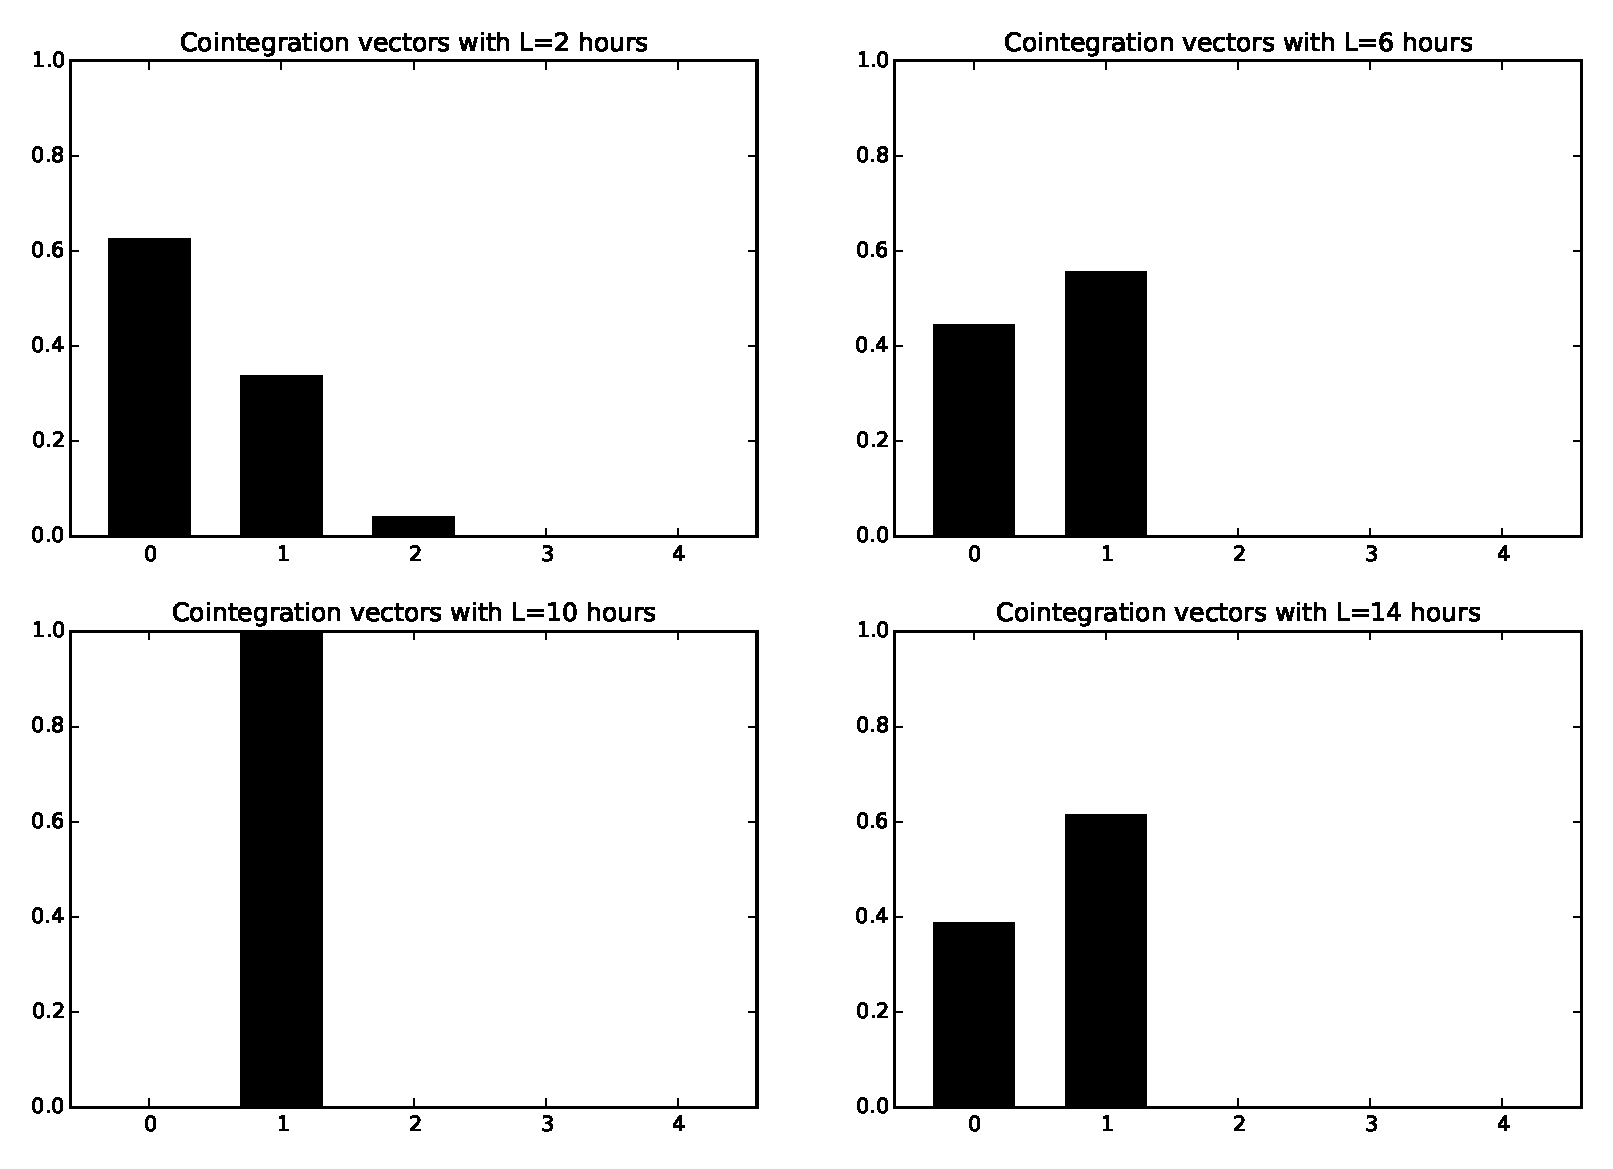
\includegraphics[width=0.9\textwidth]{img/51_Fig1}
  \caption{Distribution of the number of cointegration vectors using $p=1$ lags.
  Four possible values for windows size $L$ are shown (2, 6, 10 and 14) hours (1
  hour = 360 data points).}
  \label{fig:hists}
\end{figure}

Figure \ref{fig:hists} shows the distribution of the number of cointegration
vectors given by the Johansen method for different values of $L=[2,6,10,14]$
hours and $p=1$ . This procedure was carried out by a sliding window of
historical data moving 1000 times. We observed that the distribution of
cointegration vectors changed with different values of $L$. When
$L=2$ hours, there was no cointegration in more than 60\% of the iterations.
Cointegration increased when $L=6$ hours and was maximum when $L=10$ hours where
one cointegration vectors was found for all 1000 iterations. The ocurrence of
cointegration started to decrease at $L=14$ hours.

From section \ref{sec:vecm} we know that $r=0$ means no cointegration and
$r=l$ (we are using four rates, so $l=4$) reveals that no process is I(1) but
stationary.  The interesting cases of cointegration are those where $r$ lies
strictly between $0$ and $4$, i.e. $0<r<4$.

In order to measure the extent of cointegration, we introduce a
{\em percentage of cointegration\/} as following:
\begin{equation} \label{eq:pcoint}
PC = 
\frac{\#\{ it \mid \text{$it$ has $r$ c.v. with $0<r<l$}\}}
     {\#it}\times 100
\end{equation}
where c.v. stands for cointegration vectors and $it$ is the number of iterations.

The goal of our next experiment was to find a relationship between the ratio $PC$
and the performance measure MSE (see equation \ref{eq:MSE}). $L$ was defined
between $[2,14]$ hours, that corresponded to $[720, 5040]$ data points, and $p$
took values between $[1,5]$.  

\begin{figure}[ht!]
  \centering
   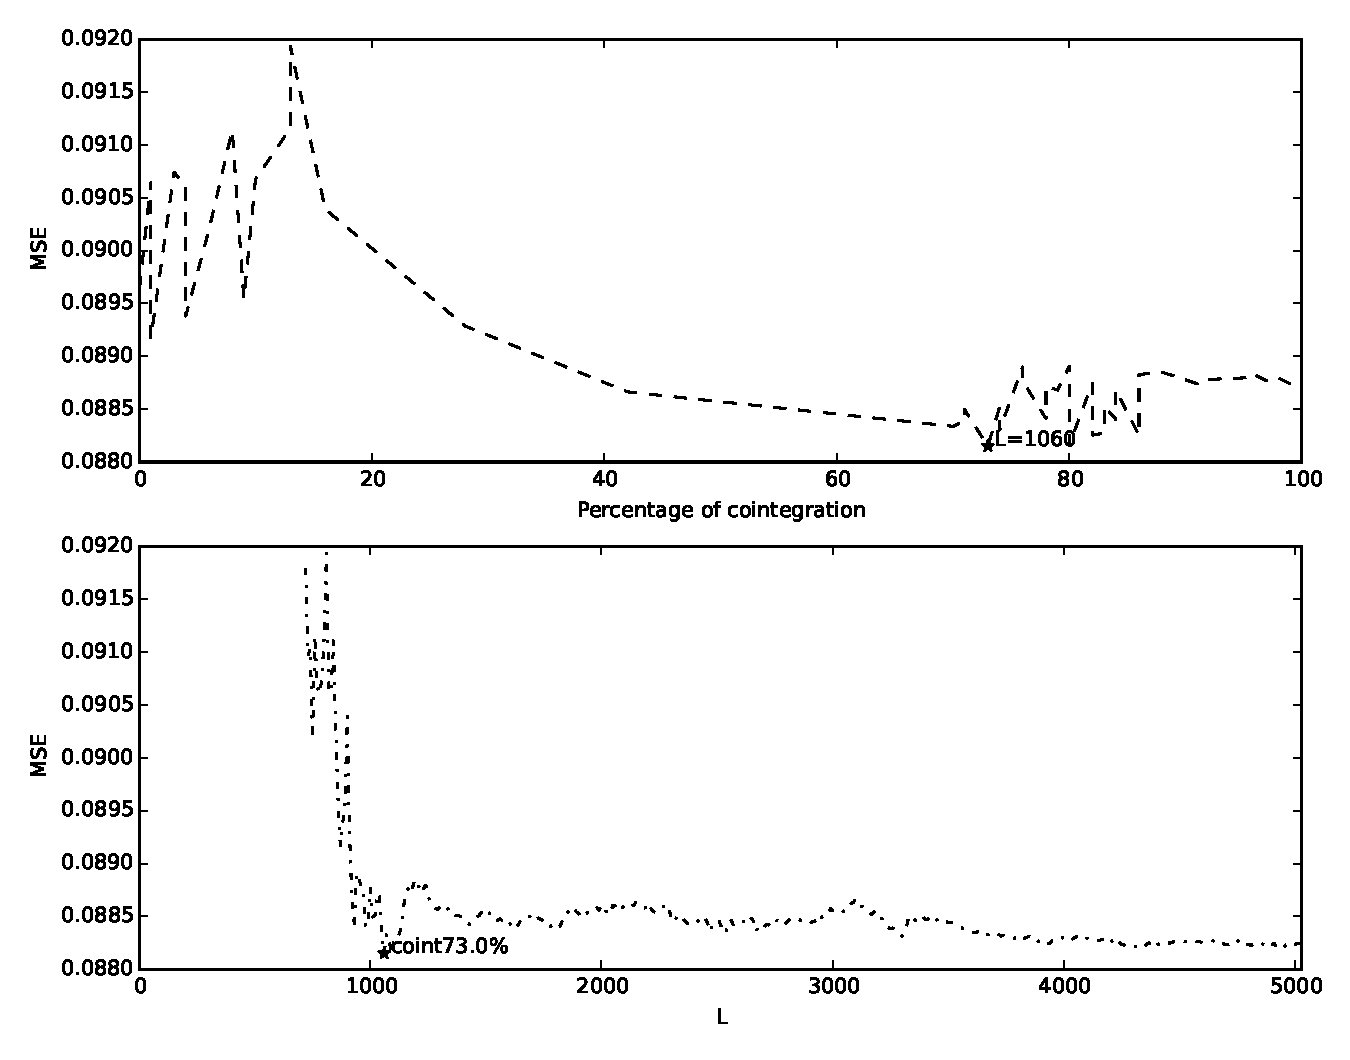
\includegraphics[width=0.9\textwidth]{img/51_Fig2}
  \caption{MSE versus the percentage of cointegration considering 1000
  iterations. Optimum windows size $L$ found was 1060. Below MSE versus $L$ shows a
  rapidly decreasing behaviour, founding minimum at PC = 73\% }
  \label{fig:cointvsmse}
\end{figure}

Figure~\ref{fig:cointvsmse} shows the relationship between MSE and $PC$ and $L$. We
found that higher cointegration percentage leads to improved performance accuracy
in terms of lower MSE. Also, increasing the size of the sliding window $L$
doesn't necessarily help to reduce MSE.

Therefore we proposed to choose $L$ and $p$ in order to maximise the percentage
of cointegration $PC$ in the near past. This process was done every time that
new data was processed. However, this search can be slow if we try different
values for $L$ and $p$ and therefore we distributed this calculation in order to
reduce searching time.

Our proposal is then a modified version of VECM, with parameter $p$ and the
amount of historical data used $L$ obtained at every step. Only the search of
$L$ and $p$ was done in a distributed environment, since this is the most
expensive routine. Our proposal is called Adaptive Vector Error Correction model
(AVECM). AVECM is detailed in the algorithm \ref{alg:AVECM} which summarises
our proposal.

\begin{algorithm}[ht!]
\begin{algorithmic}[1]
\REQUIRE $\,$ \\
$\mathbf{y}$: matrix with $N$ input vectors and $l$ time series\\
$j$: Starting point of testing \\
$it$: Ending point of testing \\
$ps$: list of $p$ values \\
$Ls$: list of $L$ values ($L<N$) \\
$m$: Iterations to determine parameters ($m < N-L$)\\
\ENSURE  $\,$ \\
$\{ \hat{\mathbf{y}}[1],\dots,\hat{\mathbf{y}}[it]\}$: prediction vectors \\
\FOR { $i =j$ to $it$ }
   \STATE $\mathbf{Y} \gets \mathbf{y}[:,i-1]$
    \STATE $L,p \gets
    \texttt{get\_best\_params}(Ls,ps,m,\mathbf{Y})$
        \STATE $model = \text{VECM}(\mathbf{Y},L, p)$
        \STATE $\hat{\mathbf{y}}[i-j] = model.predict()$
\ENDFOR
\end{algorithmic}
\caption{AVECM: Adaptive VECM.}
\label{alg:AVECM}
\end{algorithm}

The input of AVECM is time series prices which are cointegrated. The starting
point of testing is $j$ and the total number of iterations is $it$. We need to
ensure that $j$ is at least the maximum value of $Ls$. $Ls$ and $ps$ are the
possible values for $L$ and $p$.  The function {\bf get\_best\_params} makes
this grid search on the two vector lists $Ls$ and $ps$ and returns the
parameters $L$ and $p$ which maximise the percentage of cointegration $PC$ (see
equation~\ref{eq:pcoint}) for a pre-defined number of iterations $m$. This
function is implemented in a distributed environment, thus ensuring a response
before new data is available.  After $L$ and $p$ parameters are found, VECM is
built and used to forecast the next data point.


\subsection{Model comparison}
We compared our proposal, in terms of performance, with the naive forecast of
the random walk model and ARIMA. It is still difficult to outperform the random
walk model for standard econometric forecasting models  despite its
simplicity, see \cite{lo2011}. The random walk model is defined as:

\begin{equation}
\mathbf{y}_t = \mathbf{y}_{t-1} + \epsilon_{t}
\label{rwmodel}
\end{equation}

The naive forecast of the time series difference $\hat{\mathbf{y}}_{t+1}$ for
the random walk model is defined as:
\begin{equation}
\hat{\mathbf{y}}_{t+1} = \mathbf{y}_t + \hat{\epsilon}_{t+1} 
\end{equation}
\noindent where  $\hat{\epsilon}_{t+1} = \epsilon_{t}$.

On the other hand, ARIMA is widely used to forecast returns in finance, see
\cite{tsay2005}. A process can be modelled as an ARIMA$(p,d,q)$ model if
$\mathbf{x}_t=\Delta^d \mathbf{y}_t $, i.e after differencing $d$ times the time
series $\mathbf{y}_t$,  we get an ARMA$(p,q)$. Since we are modelling returns,
we used $d=1$.


\subsection{Evaluation methods}

Forecast performance was evaluated using two different methods which are
frequently used in finance:
\begin{description}
\item[MSE]  Mean Square Error measures the distance between forecasts
and the true values and large deviations from the true value have a
large impact due to squaring forecast error.
\begin{equation}\label{eq:MSE}
\text{MSE} = 
\frac{\displaystyle \sum_{t=1}^{N} (\mathbf{y}_t-\hat{\mathbf{y}}_t)^2}{N}
\end{equation}
\item[$U$-statistic] the Theil's $U$-statistic, presented by
\cite{theil1966}, is a unit free measure obtained as the ratio between the root
MSE (RMSE) of a model and the RMSE of the naive random walk model. A
$U$-statistic less than 1 implies the performance is better than the naive
model.
\end{description}


\section{Experimental results}
\label{sec:51results}
\subsection{Data}
All the experiments and AVECM tests were carried out using four foreign exchange rates all related to
USD: EURUSD, GBPUSD, USDCHF and USDJPY. We chose the most traded rates related
to USD so they were likely to be cointegrated. 
This data was collected from
\cite{Dukascopy2014}, a free database which gives access to the Swiss Foreign
Exchange marketplace.

The tests were done using 10-second frequency from ask prices from the 11th to
the 15th of August 2014. Since one day corresponds to 8640 data points and we
used 5 days of data, we have 43,200 data points in total.

\subsection{Unit root tests}

Before running the tests, we firstly checked whether the time series were I(1)
using the Augmented Dickey Fuller (ADF) test with lags $p=1,2,3,4,5$.
\cite{mackinnon2010} presented critical values for rejection of hypothesis of a
unit root: -2.62 (1\%), 1.94 (5\%) and 1.62 (10\%).
\begin{table*}[ht]
\label{tab:adf}
\centering
\begin{tabular}{llllll}
\toprule
{Variable} & {ADF(1)} & {ADF(2)} & {ADF(3)} & {ADF(4)} & {ADF(5)}\\ 
\midrule
EURUSD &  -0.052   & -0.054  & -0.054  & -0.054  & -0.054  \\
GBPUSD &  -0.744  & -0.784  & -0.805  & -0.837  & -0.846  \\
USDCHF &  -0.476   & -0.493  & -0.493  & -0.495  & -0.502  \\
USDJPY &  0.357   & 0.360  & 0.360  & 0.367  & 0.367  \\
$\Delta$ EURUSD & -128.4*  & -128.4*  & -96.85* & -89.12*   & -89.12*\\
$\Delta$ GBPUSD & -131.4*  & -112.7*  & -102.5* & -92.86*   & -88.29*\\
$\Delta$ USDCHF & -127.8*  & -127.8*  & -96.94* & -88.82*   & -80.79*\\
$\Delta$ USDJPY & -135.1*  & -135.1*  & -101.2* & -101.2*   & -101.2*\\
\bottomrule
\addlinespace[1ex]
\multicolumn{6}{l}{ \textsuperscript{*} Indicates significance at 1\% level} \\
\multicolumn{6}{l}{ \textsuperscript{**} Indicates significance at 5\% level} \\
\multicolumn{6}{l}{ \textsuperscript{***} Indicates significance at 10\% level} \\
\multicolumn{6}{l}{MacKinnon critical values for rejection of hypothesis of a unit root are:}\\
\multicolumn{6}{l}{ -2.62 (1\%), -1.94 (5\%) and -1.62 (10\%)}\\
\multicolumn{6}{l}{ADF($d$) Augmented Dickey-Fuller test with lag $d$} 
\end{tabular}
\caption{Unit roots tests for EURUSD, GBPUSD, USDCHF and USDJPY at 10-second
frequency.}
\end{table*}
Table~\ref{tab:adf} shows that all currency rates cannot reject the unit root
test in their level form considering different lags, but they rejected it with
their first differences. This means that all of them are I(1) time series and we
are allowed to use VECM and therefore our proposed AVECM.

\subsection{Performance accuracy}

Algorithms AVECM, ARIMA and the naive random walk were tested using four days of
data (from the 12th to the 15th of August 2014).  For AVECM we considered
different number of iterations (parameter $m$ in algorithm \ref{alg:AVECM}): 10,
50 and 100. We tried 12, 24 and 47 different pair of combinations for $L$ and
$p$. Possible values for $L$ were in the interval $[2,14]$ hours and $p$ can
have values in between $[1,5]$. Best AVECM performance was compared against
ARIMA and the random walk model.  Table~\ref{tab:stats} shows the out-of-sample
performance measures: MSE and $U$-statistic for AVECM and ARIMA. In terms of
both measures we found that AVECM is superior to ARIMA and the naive random walk
model. We also included the p-value that proves that the difference in the MSE
is significant at the 99\% significance level in three of the four currency
rates and at 90\% in the case of GBPUSD. The $U$-statistic shows that AVECM and
ARIMA are superior to the naive random walk model and that our proposal is also
superior to ARIMA.

\begin{table}[!htbp]
\caption{AVECM performance}
\label{tab:stats}
\begin{center}
\begin{tabular}{ccccccc}

& \multicolumn{3}{l}{MSE} & &
\multicolumn{2}{c}{$U$-statistic} \\ 
\hhline{~---~--} \\
 &
AVECM & ARIMA & p-value & &
AVECM & ARIMA \\ 

\hline
 EURUSD & 1.0702 e-09 & 1.1481 e-09 &  9.2509 e-12 & & 0.6863 & 0.7108\\
 GBPUSD & 1.6630 e-09 & 1.7408 e-09 &  6.9519 e-02 & & 0.6866 & 0.7025\\
 USDCHF & 5.8503 e-10 & 6.3545 e-10 &  2.8999 e-14 & & 0.6803 & 0.7091\\
 USDJPY  & 6.3483 e-06 & 6.5194 e-06 &  6.8536 e-05 & & 0.6964 & 0.7057\\
 \end{tabular}
 \end{center}
\end{table}

\subsection{Parallel implementation}

To determine $L$ and $p$ based on maximising the percentage of cointegration
requires use of the Johansen method which is a computationally expensive
routine. This procedure is done by the function
get\_best\_params($Ls,ps,m,\mathbf{Y}$) shown in algorithm \ref{alg:AVECM}.  In
order to improve the execution time of this search, our proposal included a
parallel search of VECM parameters using high performance computing.  The main
objective was to obtain a response before a new data arrived in the following 10
seconds.

The Johansen method is already programmed in the Python Statsmodels
library, see \cite{seabold2010}, and the parallel implementation was developed using
MPI in Python.  We chose MPI because it allows large-scale parallel applications
with wide portability to be built, being able to run in large clusters or on
local computers.  We tested our proposal in a cluster with 2 servers Xeon
E5-2667 (2.90GHz) of 24 cores each (48 cores in total) and 24GB RAM.  In order
to compare serial and parallel execution times in AVECM, we set parameter
$it=100$ in algorithm \ref{alg:AVECM}.

The $L$ parameter was always chosen between 2 and 14 hours and $p$ always took
values between 1 and 5. Parameter $nparams$ represents the number of pairs
($L$,$p$) used to maximise the percentage of cointegration. 

Execution time depends directly on $L$, $p$ and $nparams$ used, since they
determine the size of matrix $\mathbf{A}$ (see equation \ref{eq:Amatrix}) and
therefore affect the OLS function execution time.  Therefore, if we try more
combinations of $L$ and $p$ (increasing $nparams$) the serial algorithm will
take longer. For this financial time series we are interested in execution times
below 10 seconds  (the time series frequency).

\begin{figure}[ht]
  \centering
  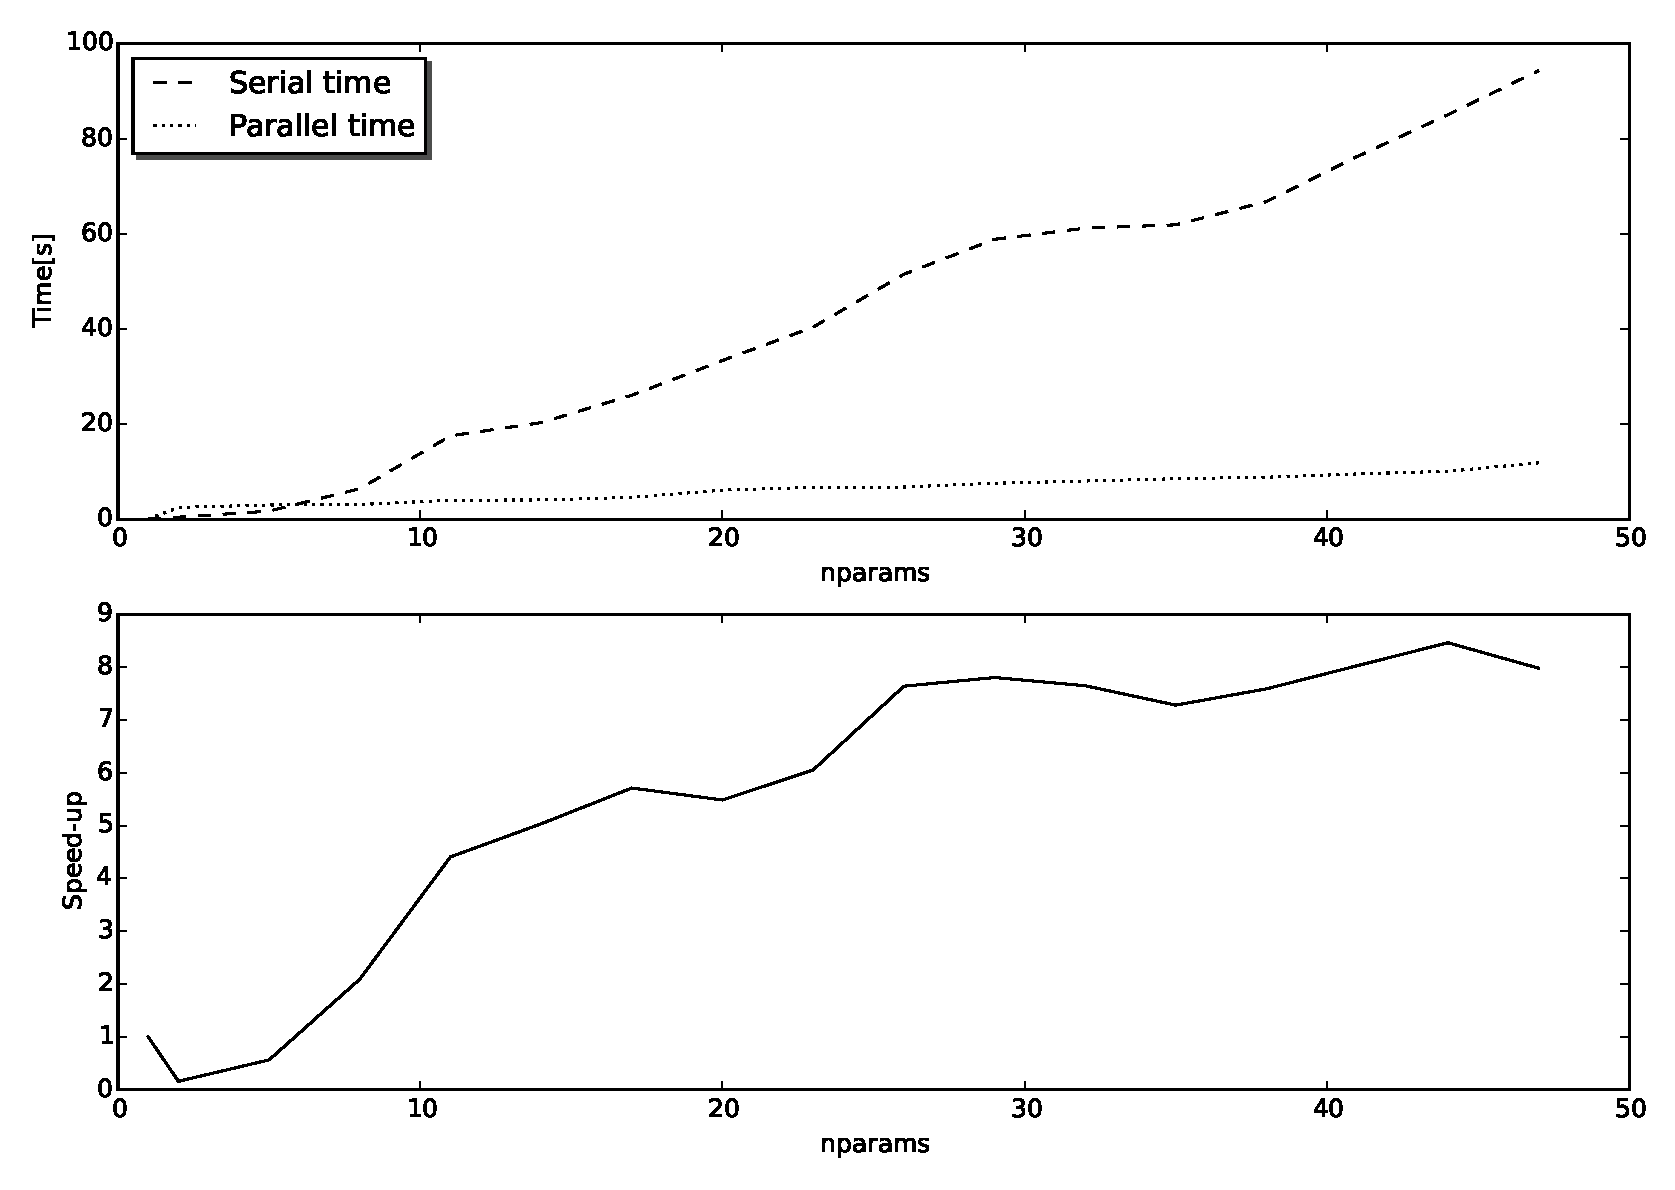
\includegraphics[width=0.9\textwidth]{img/51_Fig3}
  \caption{Computing time of sequential and parallel algorithm is shown in the
  upper figure. Speed-up is shown below.}
  \label{fig:extimes}
\end{figure}

The superior figure in \ref{fig:extimes} shows that best performance accuracy
measurements are achieved in times near or below 10 seconds in the parallel
version. Contrarily, serial times are higher, above 10 seconds in most cases.
Figure~\ref{fig:extimes} also shows the speed-up in computing time for AVECM
which is near 9X if we use more than 25 parameters ($nparams$).

Execution times do not consider the loading data time, just that of finding best
parameters and matrix operations. The time MPI spends transferring data and
synchronising processes is about two seconds independently of the number of
processes considered. Execution times were measured using the Time python
library.

\section{Conclusions}
\label{sec:51conclusions}
Cointegration in financial time series has been largely studied and the Johansen
method is commonly used to obtain cointegration relationships. In practice, it
has been found that cointegration relations change with time. However,
model-based cointegration such as VECM assumes that cointegration remains
unchanged in time. We empirically showed that the Johansen method is sensitive
to the number of lags but also to the amount of data considered.

Moreover, we introduced the notion of {\em percentage of cointegration\/} and
found that out-of-sample forecast performance MSE is related to the value of
this figure in the last samples.  We used this information to set the model
parameters.  Our proposal AVECM consists of an adaptive algorithm to update VECM
parameters every time that new data is available. These parameters are found by
maximising the percentage of cointegration of the last samples or iterations.

Despite the fact that high frequency Forex data can be spurious, the model
performance can be less reliable (and more spurious) relative to the lower
frequencies (such as 1 minute or 5 minute intervals) adopted by some other
studies. However, the deficiency is offset by gain in accuracy from parallel
processing which is capable of searching or examining a much larger state space
given the same computational time.

Determining VECM parameters was the most expensive routine and it was run using
parallel processes using MPI which allowed a grid search within a range of
values for $L$ and $p$ to be made.  Tests were done using real currency rates
data.  

Results showed that our proposed AVECM improves performance measures by finding
parameters of $L$ and $p$ maximising the percentage of cointegration. 

The parallel implementation allowed the execution times to be reduced more than
9 times and therefore a response time was obtain before 10 seconds. Since we
used 10-second frequencys we can say that our proposal is suitable for use in an
online context for real applications because response times were less than this
frequency. Cointegration information can now easily be used as an integration tool
to detect arbitrage opportunities or risk control.

For future study, it would be interesting to explore the relationship between
cointegration and performance in order to propose new criteria for improving
VECM parameters. It would also be interesting to include more explaining
variables such as bid-ask spread and change in volume.

